% Author: Damanic Luck
% Email: damanicluck@berkeley.edu
% CSM16A Fall 2023
% This question was like a fever dream to me i don't remember where the idea came from
% Author Note: This was originally suppose to include a question for how to derive least squares, but i decided it would make the worksheet too long. someone else can do it if youd like or ill revisit when im bored.

\qns{Cloudy with a Chance of Eggs}


\textbf{Learning Goal:} Build an understanding for how to arrive at the least squares formula, its applications, and how to set up the least squares solution.

\meta{
    Review block: This meta block will be deleted after review, but if it looks comprehensive enough just leave a 'lgtm' comment. if not, please write a comment for any suggestions you have that may make this question more comprehensive or clear about certain parts.
}

\meta {
    \begin{itemize}
        \item A more realistic example may be trying to provide a best for data that is showing a person's height vs shoe size.
        \item Refer to Note 23 on Least squares for the derivational portion
        \item It may be difficult for students to understand that we can apply least squares to a sinusoidal-looking graph, but as long as the model we create is linear in relation to its unknowns, we can do this. When you plug in $t$ into the proposed sinusoidal equation, the $\cos{x}$ and $\sin{x}$ functions turn into constants.
        \item This question is decently similar to Fall 2023 Final \#11 Mixed Signals. Refer to that if students want extra practice
    \end{itemize}
}

%You devise a plan to toss a carton of eggs out the window at the start of every hour starting at 6:00AM, which the last carton thrown out at 3:00PM, for a total of 10 data points. 

\begin{enumerate}

    % Question 1 %%%%%%%%%%%%%%%%%%%%%%%%%%%%%%%%%%%%%%%%%%%%%%%%%%%%%%%%%%%%%%
    \item Suppose one day inspiration strikes since your friend Bob has a magical power where eggs just appear in front of him when he wishes for them. You start wondering if you can predict how many people's attention Bob can get by tossing a carton of eggs out the window based on what time of day it is. \textbf{What's one way you could do this?} \emph{Despite Bob's amazing ability, you're limited on how many eggs he can throw out of his window since you don't want Bob to be the next WarnMe email.}
    
    \ans {
        We can sample a certain amount of data points (ie throw eggs out the window some number amount times (greater than the amount of coefficients you wish to solve for) and record the time of day). Then we can use least squares to find an appropriate model to approximate (maybe) noisy data. Keep in mind that least squares \textbf{cannot} be used in the case of an \emph{underdetermined system} since we want to ultimately minimize error between the observed value and predicted value of the solution.
    }

    % Question 2 %%%%%%%%%%%%%%%%%%%%%%%%%%%%%%%%%%%%%%%%%%%%%%%%%%%%%%%%%%%%%%
    \item Suppose Bob gets the following (noisy) data points. He has proposed a model for you and graphed it already (what a cool friend). However, can you set up this problem as a set of linear equations? If you can't, write no and then draw your best interpretation of Bob's inner thoughts. If yes, write yes and justify.
    
    \[f(t) = a_1 \cos{3t} + a_2\sin{t} + a_3\sin{0.5t} + a_4\]

    \begin{center}
    \begin{tabular}{m{4.5cm}m{10cm}}
        % {*{2}{>{\centering\arraybackslash}b{\dimexpr0.5\linewidth-2\tabcolsep\relax}}}
        \begin{center}
            \begin{tabular}{c|c|c}
                Point & $t$ & $f(t)$ \\
                \hline
                0 & 0 & 6.2 \\
                1 & 0.5 & 4.6 \\
                2 & 1 & 3.8 \\
                3 & 1.5 & 7.4 \\
                4 & 2 & 9\\
                5 & 3 & 4.1 \\
                6 & 3.5 &  3.5\\
                7 & 4 & 5.4 \\
                8 & 4.5 & 3.4 \\
            \end{tabular}
        \end{center}
        &
        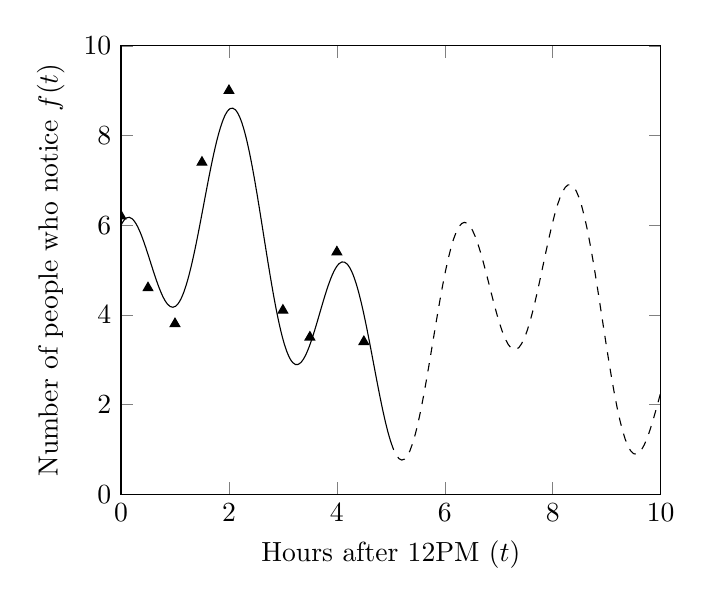
\begin{tikzpicture}
            \begin{axis}[
              xlabel= Hours after 12PM $(t)$,
              ylabel= Number of people who notice $f(t)$,
              xmin=0,
              xmax=10,
                ymin=0,
                ymax=10
            ]
                \addplot [samples=100,smooth,no markers,domain=0:5] {2*cos(deg(3*x))+2*sin(deg(x))+sin(deg(0.5*x))+4};
                \addplot [samples=100,dashed,no markers,domain=5:10] {2*cos(deg(3*x))+2*sin(deg(x))+sin(deg(0.5*x))+4};
                \node[color=black,scale=1]  at (axis cs:0, 6.2) {\(\pgfuseplotmark{triangle*}\)};
                \node[color=black,scale=1]  at (axis cs:0.5, 4.6) {\(\pgfuseplotmark{triangle*}\)};
                \node[color=black,scale=1]  at (axis cs:1, 3.8) {\(\pgfuseplotmark{triangle*}\)};
                \node[color=black,scale=1]  at (axis cs:1.5, 7.4) {\(\pgfuseplotmark{triangle*}\)};
                \node[color=black,scale=1]  at (axis cs:2, 9) {\(\pgfuseplotmark{triangle*}\)};
                \node[color=black,scale=1]  at (axis cs:3, 4.1) {\(\pgfuseplotmark{triangle*}\)};
                \node[color=black,scale=1]  at (axis cs:3.5, 3.5) {\(\pgfuseplotmark{triangle*}\)};
                \node[color=black,scale=1]  at (axis cs:4, 5.4) {\(\pgfuseplotmark{triangle*}\)};
                \node[color=black,scale=1]  at (axis cs:4.5, 3.4) {\(\pgfuseplotmark{triangle*}\)};
            \end{axis}

        \end{tikzpicture}
    \end{tabular}
    \end{center}

    \ans{
        Yes, you can write these sample points with the proposed model in a set of linear equations. If you plug in the value of $t$ and $f(t)$, sines and cosines here become scalars next to our unknown coefficients.
    }
    % Question 3 %%%%%%%%%%%%%%%%%%%%%%%%%%%%%%%%%%%%%%%%%%%%%%%%%%%%%%%%%%%%%%
    \meta{
        Establishing constraints for least squares for this question onward and then solving for this for the unknowns.
    }

    \item Regardless of your answer from part(2), suppose that we can use least squares on Bob's proposed model. How can you modify his proposed model so that we \textbf{cannot} apply least squares? 
    
    \ans {
        In order to make it such that we \emph{cannot} apply least squares, the equations that we can set up from from the proposed model and the sample data \emph{should not} be linear. There are multiple answers for this section. One way of making the proposed model produce non-linear equations would be to insert another coefficient to solve for within one of the sine or cosine equations. Such as \dots 
        \[f(t) = a_1 \cos{(3 \cdot \textcolor{green}{b} \cdot t)} + a_2\sin{t} + a_3\sin{0.5t} + a_4\]
        or
        \[f(t) = a_1 \cos{3t} + a_2\sin{(t \cdot \textcolor{green}{b})} + a_3\sin{0.5t} + a_4\]
    }

    % Question 4 %%%%%%%%%%%%%%%%%%%%%%%%%%%%%%%%%%%%%%%%%%%%%%%%%%%%%%%%%%%%%%
    \meta{
        The main takeaway should be $A^TA$ is invertible if $A$ is linearly independent.
    }

    \item Bob is actually really interested in least squares today! Below, the least squares solution for $A\vec{x} \approx \vec{b}$ is written for convenience. Is $A^T A$ invertible, given that $A$ is linearly independent? Write a proof for this. \emph{Hint: What conclusions can we draw from $A$ being linearly independent?}
    \[\vec{\hat{x}} = (A^T A)^{-1} A^T \vec{b}\]
    
    \ans{
        \textcolor{magenta}{$\star$ As a note, the actual contents of this proof will walk you through it and try to provide as many clarifications as possible. However, it's unecessary to write out this much. Because of this, side note paragraphs will be colored in magenta and marked with a star symbol.}

        Since we know that $A$ is linearly independent, we know that the nullspace of $A$ is trivial, so 
        \[\mathrm{Null}(A) = \vec{0}\]
        \textcolor{magenta}{$\star$ Another way to think about this is to think of all values of $\vec{x}$ that make the following equation true: 
        \[A\vec{x}=\vec{0}\]}
        \textcolor{magenta}{$\star$ Keep in mind that $A$ may not necessarily be square, so let it be of dimension $n \times k$, where $n$ may or may not be equal to $k$. However, when left multiplying $A$ by its transpose, this will result in a square matrix. As a sanity check, we can write out the dimensions of $A^T$ and $A$, which are $k \times n$ and $n \times k$ respectively. We see here that the dimension of the resulting matrix is $k \times k$, which is a square matrix as desired. Keep in mind that a square matrix with a trivial nullspace means it is invertible.}
        
        We consider an arbitary $\vec{v} \in \mathrm{Null}(A^TA)$. Since $\vec{v}$ lives in the nullspace of $A^TA$, this means that 
        \[A^TA \vec{v} = \vec{0}\]
        Multiply both sides of this equation by $\vec{v}^T$. 
        \[\vec{v}^T A^T A \vec{v} = \vec{v}^T \vec{0} = 0\]
        \textcolor{magenta}{$\star$ Notice that when we multiply the the zero vector by $\vec{v}^T$ that this turns into the \textbf{scalar} zero. This is because we can think of $\vec{v}^T \vec{0}$ as the inner product between $\vec{v}$ and the zero vector. We want to multiply both sides by $\vec{v}^T$ in order to write out the left side as an inner product. Keep in mind that ultimately we want to relate this back to the nullspace of $A$ as well.}
        
        \textcolor{magenta}{$\star$ Remember the following:
        \[(A\vec{v})^T = \vec{v}^T A^T\]
        You can perform another sanity check by checking the dimensions here. If $A$ is a $n \times k$ matrix and $\vec{v}$ is a $k \times 1$ vector, then $(A\vec{v})^T$ is of dimension $1 \times n$. Carrying out the same thought process on the right hand side results in the same dimension column vector as the right hand side.}


        Simplifying the left hand side yields:
        \[(A\vec{v})^T (A\vec{v}) = 0\]

        \textcolor{magenta}{$\star$ The following properties are useful to remember for the next part
            \begin{align*}
                \langle x , \; x \rangle &= ||x||^2 \\
                \langle x , \; x \rangle &= 0 ~\mathrm{IFF} x = 0
            \end{align*}
        }
        By definition of an inner product, the above implies the following:
        \[ \langle A\vec{v} \; , \; A\vec{v} \rangle  = ||A\vec{v}||^2 = 0\]

        \textcolor{magenta}{$\star$ To prove that Null($A$) = Null($B$), you must prove both directions meaning that you must prove that Null($A) \subseteq$ Null($B$) (which is read as "the nullspace of $A$ is a subset of the nullspace of $B$" (ie, vectors that exist in $\mathrm(Null)(A)$ also exist in $\mathrm(Null)(B)$)) and Null($B) \subseteq$ Null($A$). In the following steps, you'll see that its was more difficult to prove one direction over the other.}

        We can see after simplifying that $A\vec{v} = 0$. This means that $\vec{v} \in \mathrm{Null}(A)$. Earlier, we stated that $\vec{v} \in \mathrm{Null}(A^TA)$, so therefore $\mathrm{Null}(A^TA) \subseteq \mathrm{Null}(A)$

        Now suppose we have a vector, $\vec{v'}$, where $\vec{v'} \in \mathrm{Null}(A)$, so 
        \[A\vec{v'} = \vec{0}\]
        Left multiplying by $A^T$ results in 
        \[A^TA\vec{v'} = \vec{0}\]
        We can conclude that 
        \[\mathrm{Null}(A) = \mathrm{Null}(A^TA)\]
    }
    % Question 6 %%%%%%%%%%%%%%%%%%%%%%%%%%%%%%%%%%%%%%%%%%%%%%%%%%%%%%%%%%%%%%
    \item From the previous part, how can we derive our general least squares solution? \emph{Hint: Our starting point here is $A\vec{x} = \vec{b}$, where $A$ is not always square. you know that there exists an inverse for $A^TA$.}
    
    \ans {
        \begin{align*}
            A\vec{x} &= \vec{b} \\
            A^TA \vec{x} &= A^T \vec{b} \\
            (A^TA)^{-1} A^T A \vec{x} &= (A^T A)^{-1} A^T \vec{b} \\
            \vec{x} &= (A^TA)^{-1} A^T \vec{b}
        \end{align*}
    }
    % Question 7 %%%%%%%%%%%%%%%%%%%%%%%%%%%%%%%%%%%%%%%%%%%%%%%%%%%%%%%%%%%%%%
    \item How many unknowns do you have to solve for? Which ones? Bob's proposed model has been recopied here for convenience.
    \[f(t) = a_1 \cos{3t} + a_2\sin{t} + a_3\sin{0.5t} + a_4\]
    
    \ans {
        We have 4 unknowns to solve, which are $a_1, a_2, a_3$, and $a_4$.
    }

    % Question 8 %%%%%%%%%%%%%%%%%%%%%%%%%%%%%%%%%%%%%%%%%%%%%%%%%%%%%%%%%%%%%%
    \item From the previous part, you know how many unknowns there are! Set up the sample points, with the proposed model from part(2) as a matrix-vector equation here (in the form of $A\vec{x} = \vec{b}$).  
    
    \ans {
        \[
        \begin{bmatrix}
            \cos{(3 \cdot 0)} & \sin{(0)} & \sin{(0.5 \cdot 0)} & 1 \\
            \cos{(3 \cdot 0.5)} & \sin{(0.5)} & \sin{(0.5 \cdot 0.5)} & 1 \\
            \cos{(3 \cdot 1)} & \sin{(1)} & \sin{(0.5 \cdot 1)} & 1 \\
            \cos{(3 \cdot 1.5)} & \sin{(1.5)} & \sin{(0.5 \cdot 1.5)} & 1 \\
            \cos{(3 \cdot 2)} & \sin{(2)} & \sin{(0.5 \cdot 2)} & 1 \\
            \cos{(3 \cdot 3)} & \sin{(3)} & \sin{(0.5 \cdot 3)} & 1 \\
            \cos{(3 \cdot 3.5)} & \sin{(3.5)} & \sin{(0.5 \cdot 3.5)} & 1 \\
            \cos{(3 \cdot 4)} & \sin{(4)} & \sin{(0.5 \cdot 4)} & 1 \\
            \cos{(3 \cdot 4.5)} & \sin{(4.5)} & \sin{(0.5 \cdot 4.5)} & 1 
        \end{bmatrix}
        \begin{bmatrix}
            a_1 \\ a_2 \\ a_3 \\ a_4
        \end{bmatrix}
        = 
        \begin{bmatrix}
            6.2 \\ 4.6 \\ 3.8 \\ 7.4 \\ 9 \\ 4.1 \\ 3.5 \\ 5.4 \\ 3.4
        \end{bmatrix}
        \]
    }

    % Question 9 %%%%%%%%%%%%%%%%%%%%%%%%%%%%%%%%%%%%%%%%%%%%%%%%%%%%%%%%%%%%%%
    \item Suppose that the least square solution for this model is given by the following equation. What is the predicted number of people who will notice Bob throwing eggs out the window at 12AM? 
    \[f(t) = 2 \cos{3t} + 2\sin{t} + \sin{0.5t} + 4\]
    
    \ans {
        You can leave your answer within the sine and cosine functions without simplifying. However, if you do simplify, we see that $f(12) = 2.392$. So about 2 people will notice. 
    }
\end{enumerate}
